\chapter{Discrete Element Method}

It is a numerical method introduced by Cundall and Strack \citep{CS79}
used to model the behavior of large number of particles having finite
mass and radius which interact at their surfaces. The governing
equation of motion for such a particle can be written using Newton's
laws.

\begin{align}
  \label{eq:newton_equation_of_motion}
  \frac{d^2 \vec{x}}{dt^2} = \vec{F}(\vec{x}, \vec{v}, m)\\
  \frac{d^2 \vec{\omega}}{dt^2} = \vec{M}(\vec{x}, \vec{v}, m)
\end{align}

Where $\vec{F}$, $\vec{M}$ is the force and moment acting on the
particle. m, $\vec{v}$, $\vec{x}$ are the mass, position and velocity
of the particle.
The force $\vec{F}$ in equation\ref{eq:newton_equation_of_motion} is
the one to be computed during each time step. This force arises due to
collision of particles.

% \begin{figure}
%   \centering
%   \includegraphics[scale=0.5]{dem/two_pars_in_contact}
%   \caption{Two spherical particles in contact}
%   \label{fig:tspc}
% \end{figure}

Before studying the interaction of a particle with wall or any other
spherical particle, lets consider a spherical particle with mass m
freely falling under gravity. For such a model, the governing
differential equation can be written as

\begin{align}
  \label{eq:free_fall}
  \frac{d^2 \vec{x}}{dt^2} = \vec{g}\\
  \frac{d^2 \vec{\omega}}{dt^2} = 0
\end{align}

Such a differential equation \eqref{eq:free_fall} governs a scene like
in figure \eqref{fig:free_fall}

\begin{figure}
\centering
\begin{subfigure}{.5\textwidth}
  \centering
  \includegraphics[scale=0.3]{dem/free_fall}
  \caption{A freely falling Sphere}
  \label{fig:free_fall}
\end{subfigure}%
\begin{subfigure}{.5\textwidth}
  \centering
  \includegraphics[scale=0.3]{dem/bounce_back}
  \caption{A freely falling Sphere onto a wall}
  \label{fig:bounce_back}
\end{subfigure}
\caption{Behaviour of sphere under different conditions}
\label{fig:sphere_intro}
\end{figure}


In freely falling situation, the particle doesn't see any obstacles,
and follows a straight line path.

Now assume that there is a wall obstructing the motion of this
spherical ball.  As the ball hits the wall it has to bounce back
\eqref{fig:bounce_back}, because of the repulsion force from the
wall. There are two ways to model such a behavior.

\begin{itemize}
\item Event driven method (hard particles)
\item Discrete element methods (soft particles)
\end{itemize}


Present work deals with Discrete element method, with a little introduction
to Event driven method.

\section{Discrete element method (DEM)}
\label{sec:edm}

In this method at every instant of time the ball is checked if it is
in contact with any other particle or wall. If it is, then the force
is computed from the relative positions of the overlapping
particles. By using such force($\vec{F}$) \eqref{eq:newton_equation_of_motion} is
integrated using Euler or ARK2.

\subsection{Force calculation}
\label{sec:force}

\begin{figure}
  \centering
  \includegraphics[scale=0.5]{dem/collision}
  \caption{Two spherical particles in contact}
  \label{fig:tspc}
\end{figure}

\begin{equation}
  \label{eq:overlap}
  \delta = (r_i + r_j) - |\vec{X}_{i} - \vec{X}_{j}|
\end{equation}

Say two particles \eqref{fig:tspc} i and j with radii $r_{i}$ and
$r_{j}$, are in contact if $\delta$ \eqref{eq:overlap} is positive.
The particle i has linear velocity $\vec{V}_{i}$ and angular velocity
of $\vec{\omega}_{i}$ particle j has linear velocity $\vec{V}_{j}$ angular
velocity of $\vec{\omega}_{j}$.

The unit normal vector along particle i to particle j  is given by

\begin{equation}
  \label{eq:normal_unit}
  \vec{n}_{ij} = \frac{\vec{X}_{j} - \vec{X}_{i}}{|\vec{X}_{j} - \vec{X}_{i}|}
\end{equation}

The relative velocity of point of contact becomes

\begin{equation}
  \label{eq:relative}
  \vec{V}_{ij} = \vec{V}_{i} - \vec{V}_{j} +
  (r_{i} \vec{\omega}_{i} + r_{j} \vec{\omega}_{j}) \times \vec{n}_{ij}
\end{equation}

Therefore the normal and tangential components of contact velocity are

\begin{equation}
  \label{eq:normal_vel}
  \vec{V}_{nij} = \vec{V}_{ij} \cdot \vec{n}_{ij} \vec{n}_{ij}
\end{equation}

\begin{equation}
  \label{eq:tang_vel}
  \vec{V}_{tij} = \vec{V}_{ij} - \vec{V}_{ij} \cdot \vec{n}_{ij} \vec{n}_{ij}
\end{equation}

The tangent to the plane of contact is

\begin{equation}
  \label{eq:tang_unit}
  \vec{t}_{ij} = \frac{\vec{V}_{tij}}{|\vec{V}_{tij}|}
\end{equation}


Discrete element method is a soft sphere approach. In soft sphere
approach the overlap between two particles is described by a spring
and a dashpot in both normal and tangential direction. Generally, when
two particles collide, there will be a repulsion force on both the
particles. This repulsive force is represented by springs, whose
magnitude depends on the overlap amount. Similarly, when a collision
occurs, there will be damping of energy due to deformation of the body
and the friction force between the particles. This damping is taken
care by the dashpot between the particles. The respective spring and
damping coefficients depend on the coefficient of restitution between
the colliding particles and the material properties of the colliding
particles.


The normal ($\vec{F}_{nij}$) and tangential ($\vec{F}_{tij}$)
components of the contact force ($\vec{F}_{ij}$) at time t can be
written as

\begin{equation}
  \label{eq:normal_force}
  \vec{F}_{nij} =  \vec{F}_{nij}^S +  \vec{F}_{nij}^D
\end{equation}

\begin{equation}
  \label{eq:tangential_force}
  \vec{F}_{tij} =  \vec{F}_{tij}^S +  \vec{F}_{tij}^D
\end{equation}

In a linear force, normal spring force $\vec{F}_{nij}$ is computed from the overlap
amount between the particles. This force is always repulsive in nature
and it conserves the energy of the colliding particles.

\begin{equation}
  \label{eq:normal_spring_force}
  \vec{F}_{nij}^S = -k_n \> \delta_n \> \vec{n}_{ij}
\end{equation}

Since as discussed, when two particle collide there will be loss in
energy due to friction, body deformation, rolling friction and many
more. To model such energy loss, we consider a single damping force,
which depends on the coefficient of restitution between particles, and
the force opposes the velocity. Such damping force can be written as

\begin{equation}
  \label{eq:normal_damping_force}
  \vec{F}_{nij}^D = -\eta_n  (\vec{V}_{ij} \cdot \vec{n}_{ij}) \> \vec{n}_{ij}
\end{equation}


Tangential spring force is calculated in a different way. At the
instantiation of the a spring is attached in tangential direction, and
as time proceeds, the elongation of the spring is noted. At every time
step depending on the displacement of the spring the force is
computed.

\begin{equation}
  \label{eq:tang_spring_force}
  \vec{F}_{tij}^S = -k_t \> \vec{\delta_t}
\end{equation}

Where $ \vec{\delta_t} $ at the instantiation of the contact
can be written as

\begin{equation}
  \label{eq:tang_disp}
 \vec{\delta_t} = \vec{V}_{tij} \> \Delta t
\end{equation}

And after time $\Delta t$

\begin{equation}
  \label{eq:tang_disp}
 \vec{\delta}_{t + \Delta t} = \vec{\delta}_{t} + \vec{V}_{tij} \> \Delta t
\end{equation}

Where as tangential damping force is similar to normal damping force, which can be
written as

\begin{equation}
  \label{eq:tang_damp_force}
  \vec{F}_{tij}^D = -\eta_t \> \vec{V}_{tij}
\end{equation}

With such a tangential law, the force opposing the motion will increase indefinitely,
to make it finite, Coloumb condition is applied. It is given as follows

\begin{equation}
  \label{eq:coloumb}
  |\vec{F}_{tij}| > \mu \> |\vec{F}_{nij}|
\end{equation}

where $\mu$ is coefficient of friction.

\subsection{Computing normal and tangential coefficients}

We defined the force laws between two colliding spheres, these forces are
dependent on the spring and dashpot coefficients. These are computed as follows,
Generally while defining collision, material properties and coefficient of restitution is
specified, using these values, we need to come up with the coefficients.

In linear force model from MFIX DEM we have normal coefficient of restitution as
\begin{equation}
  \label{eq:damping_coefficient}
  \eta_{n} = \frac{2 \> \sqrt{m_{eff}k_{n}}|\ln e_n|}{\sqrt{\pi^2 + \ln^2e_{n}}}
\end{equation}


\section{Particle Wall collision}
\label{sec:PWColl}

Till now particle  collision is modelled. Particle wall
collision can be modelled in the following way. A point and normal to
the wall is need to be defined \ref{fig:wall_description}

\begin{figure}
  \centering
  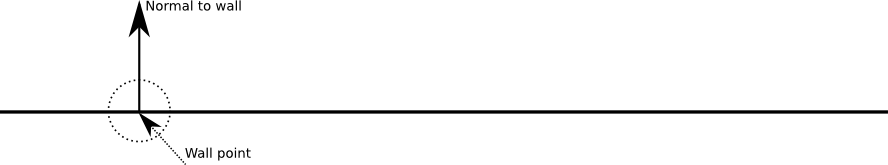
\includegraphics[scale=2.]{dem/wall_description}
  \caption{Describing a wall in DEM Simulation}
  \label{fig:wall_description}
\end{figure}


After defining a wall, to check if a given particle of radius r in
contact with the Paine the following condition is to be satisfied.

Say that $\vec{n}_w$ is the normal for wall, and the vector joining
the wall point and the particle is $\vec{r}_{wi}$. The perpendicular
distance between wall and the particle can be computed using

\begin{align}
  \label{eq:perpendicular_dist}
    Perpendicular Distance(PR) =  \vec{r}_{wi} \cdot  \vec{n}_w
\end{align}

If $r - PR $ is positive, then the particle is overlapping the wall,
such $r - PR$ is the overlap amount. Where $r$ is the radius of the
particle\ref{fig:particle_wall_collision}. From such overlap amount
and material properties force on the particle can be computed using
\eqref{eq:normal_force} and \eqref{eq:tangential_force}

\begin{figure}
  \centering
  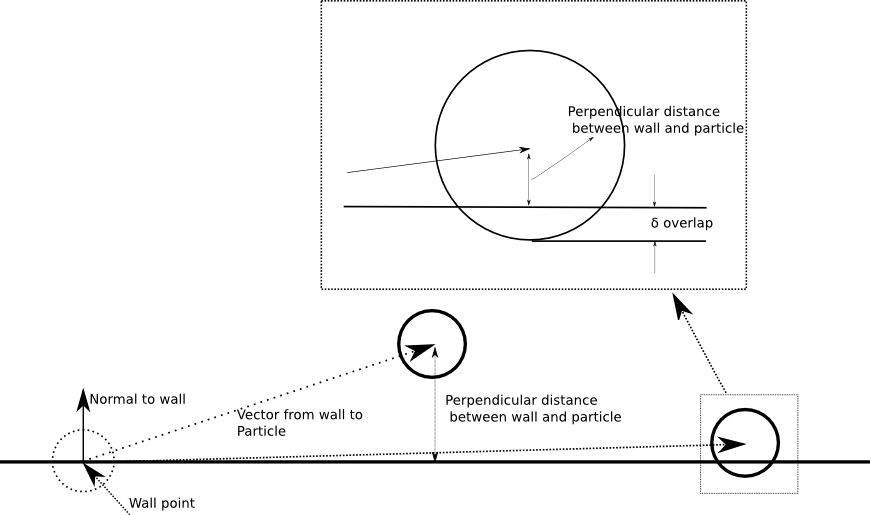
\includegraphics[scale=1.5]{dem/particle_wall_collision.png}
  \caption{Particle and wall colliding}
  \label{fig:particle_wall_collision}
\end{figure}


\section{Rigid body dynamics modelling using DEM}
\label{sec:rigid_body_dem}

Till now modelling of distinct particles is discussed. This method could be
extended to model rigid body collisions seamlessly. In the present work
2d rigid body dynamics is studied and discussed.

Physically, rigid body has a continuous mass(M) with arbitrary shape.


%%


%%% Local Variables:
%%% mode: latex
%%% TeX-master: "../mainrep"
%%% End:

%  LocalWords:  discretized
